\section{Task 3: RF Jamming Attack} \label{ch:pentesting:rf-jamming}
This section covers a pentest of a jamming attack against the RF communication in the system. This is a \gls{DOS} attack which if successful blocks or interferes with the RF communication between two devices, making them unable to send messages to each other.

\subsubsection{Background}
Many wireless communication mediums are vulnerable to jamming attacks. Radio frequency communication is certainly one of them. A jamming attack against RF communication involves directing electromagnetic energy in one or more radio frequencies against a system to disrupt or prevent signals from being transmitted between two systems \cite{adamy2004ew}. In practice, this means sending out signals on a specific frequency, carrying enough energy to overpower any one transmission in the same frequency band. By continuously sending out signals, such that the wireless band is filled, legitimate traffic can be blocked. Since RF communication uses a shared medium, this is an attack vector which can be incredibly hard to protect against. Often a system will communicate on a single, fixed frequency which can make the system particularly vulnerable to jamming attacks \cite{jamming-feasibility}.

\subsubsection{Method}
To transmit signals the HackRF SDR was used. It was placed close to the system, within \texttt{10-20 cm}. See section \ref{ch:pentesting:lab-setup} for a detailed description of the lab setup. To generate a jamming signal the open source program \textit{GnuRadio Companion}\footnotelink{https://www.gnuradio.org/}{2021-05-22}, version \texttt{3.9.0.0}, was used. This is a graphical tool used to control an SDR. It is based on creating flowgraphs of connected components to receive, process, modify, and transmit real time radio signals from and to an SDR.
\begin{figure}[!ht]
    \centering
    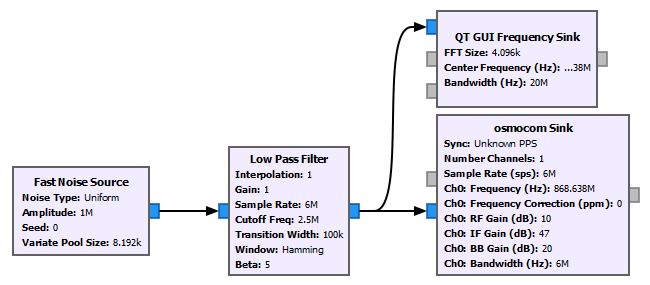
\includegraphics[width=\textwidth]{images/6-pentesting/jamming-flowgraph.png}
    \caption{A flowgraph in GnuRadio which performs a jamming attack.}
    \label{fig:gnuradio-jamming-flowgraph}
\end{figure}
To generate a noise signal, a flowgraph was created in GnuRadio Companion, see figure \ref{fig:gnuradio-jamming-flowgraph}. Initially, a \texttt{Fast Noise Generator} was used as the source signal. The output was then linked to a low-pass filter, to concentrate the signals to the specific frequency band of interest. Lastly, the output was sent to the HackRF via the \texttt{osmocom Sink} block. Additionally, the output from the low-pass filter was also sent to a \texttt{QT GUI Frequency Sink} to visually present the sent signal data while performing the attack. This is shown in figure \ref{fig:gnuradio-frequency-graph}.
\begin{figure}[!ht]
    \centering
    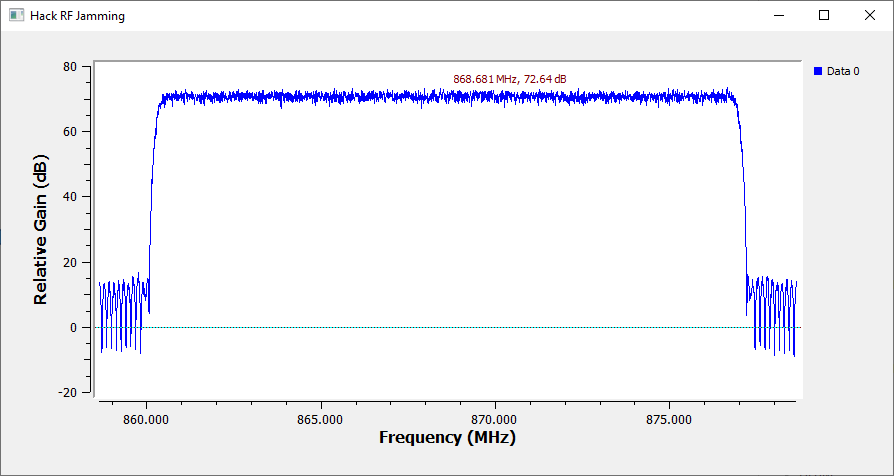
\includegraphics[width=\textwidth]{images/6-pentesting/jamming-output-graph.png}
    \caption{A frequency graph from GnuRadio during the jamming attack.}
    \label{fig:gnuradio-frequency-graph}
\end{figure}

\subsubsection{Results}
This pentest was successful. \todo.

\subsubsection{Discussion}
\todo
